\documentclass{beamer}

\usepackage{predavanja}

\usepackage{amsmath}
\usepackage{amsfonts}

\usepackage{tikz}
\usetikzlibrary{math}

\usepackage{pgfplots}
\usepgfplotslibrary{external}

\usepackage{array}

\theoremstyle{definition}
\newtheorem{definicija}{Definicija}[section]

\theoremstyle{plain}
\newtheorem{izrek}{izrek}

\newcommand{\ZZ}{\mathbb{Z}}
\newcommand{\RR}{\mathbb{R}}
\newcommand{\CC}{\mathbb{C}}

\begin{document}

\title{Matematični izrazi in uporaba paketa \texttt{beamer}}
\subtitle{\emph{Matematičnih} nalog ni treba reševati!}
\institute{Fakulteta za matematiko in fiziko}
\date{}


\begin{frame}
    \frametitle{Kratek Pregled}
    \tableofcontents %[pausesections]
\end{frame}

\section{Paket \texttt{beamer}}

\input{prosojnice/1-paket-beamer.tex}

\section{Paketa \texttt{amsmath} in \texttt{amsfonts}}

\input{prosojnice/2-paketa-amsmath-amsfonts.tex}

\section[Matematika, 1. del\\\large{Analiza, logika, množice}]{Matematika, 1. del}

\input{prosojnice/3-analiza-logika-mnozice.tex}

\section{Stolpci in slike}

\begin{frame}{Konstrukcija pravokotnice na premico $p$ skozi točko $T$}
	\begin{columns}
		\begin{column}{0.55\textwidth}
		  \begin{itemize}
			 \item<1-> Dani sta premica $p$ in točka $T$.
			 \item<2-> Nariši lok $k$ s središčem v $T$.
			 \item<3-> Premico $p$ seče v točkah $A$ in $B$.
			 \item<4-> Nariši lok $m$ s središčem v $A$.
			 \item<5-> Nariši lok $n$ s središčem v $B$ in z enakim polmerom.
			 \item<6-> Loka se sečeta v točki $C$.
			 \item<7-> Premica skozi točki $T$ in $C$ je pravokotna na $p$.
		  \end{itemize}
		\end{column}
		\begin{column}{0.45\textwidth}
			\centering
				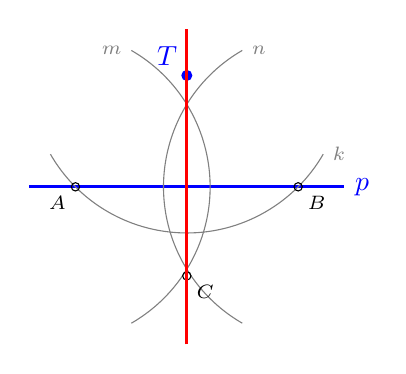
\begin{tikzpicture}
				\tikzmath{
					% Razdalja od točke T do premice p je tako 2*sin(45°).
					\t = 2*sin(45);
					% Razdalja začetka loka m do premice p
					% oz. razdalja točke T' levo in zgoraj od točke T do premice
					\tt = 2*sin(60);
					% Razdalja točke T' od navpične premice skozi T
					\td = \t-2*cos(60);
				}
				\coordinate [label={[blue, above left]:$T$}] (T) at (0,{\t});
				\fill[blue] (T) circle (2pt);
				\draw[blue, very thick] (-2,0) -- (2,0) node[right] {$p$};
				\pause
				\coordinate (A') at ({-\tt},{\td});
				\draw[gray, thin] (A') arc[start angle=210, end angle=330, radius=2] node[right] {\scriptsize $k$};
				\pause
				\coordinate [label=below left:{\scriptsize $A$}] (A) at ({-\t},0);
				\draw (A) circle (1.5pt);
				
				\coordinate [label=below right:{\scriptsize $B$}] (B) at ({\t},0);
				\draw (B) circle (1.5pt);
				\pause
				\coordinate (T') at ({-1.7*\td},{\tt});
				\draw[gray, thin] (T') node[left] {\scriptsize $m$} arc[start angle=60, end angle=-60, radius=2]; 
				\pause
				\coordinate (T'') at ({1.7*\td},{\tt});
				\draw[gray, thin] (T'') node[right] {\scriptsize $n$} arc[start angle=120, end angle=240, radius=2];
				\pause
				\coordinate [label=below right:{\scriptsize $C$}] (C) at (0, {-0.8*\t});
				\draw (C) circle (1.5pt);
				\pause
				\draw[red, very thick] (0,-2) -- (0,2);
			\end{tikzpicture}
		\end{column}
	\end{columns}

\end{frame}


% Naloga 4
\begin{frame}{Graf funkcije s TikZ}
	\centering
	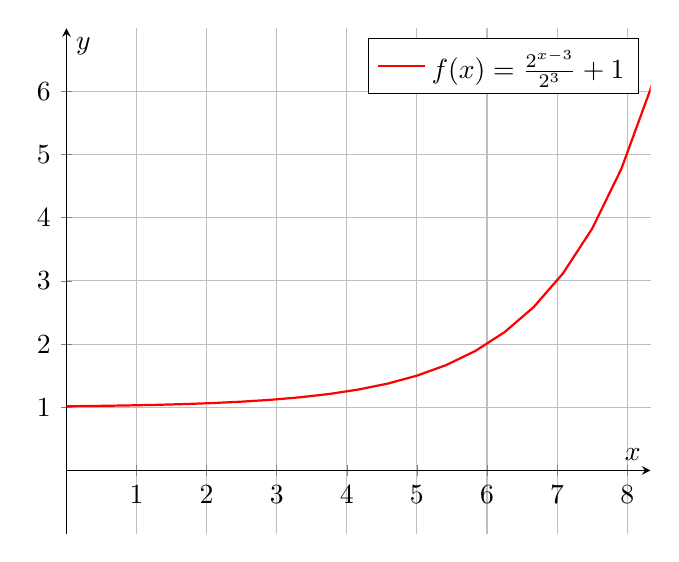
\begin{tikzpicture}
		\begin{axis}[
			axis lines = middle,
			domain = 0:10,
			width = 9cm,
			height = 8cm,
			xtick = {0, 1, 2, 3, 4, 5, 6, 7, 8},
			ytick = {0, 1, 2, 3, 4, 5, 6},
			ymin = -1,
			ymax = 7,
			grid = both,
			xlabel = {$x$},
			ylabel = {$y$}
		]
		\addplot[red, thick]{2^(x - 3)/2^3 + 1};
		\addlegendentry{$f(x) = \frac{2^{x-3}}{2^3}+1$}
		\end{axis}
	\end{tikzpicture}
\end{frame}




% % slike:
% \begin{column}{0.45\textwidth}
% \centering
% \includegraphics<1>[width=50mm]{slike/fig-1.png}%
% \includegraphics<2>[width=50mm]{slike/fig-2.png}%
% \includegraphics<3>[width=50mm]{slike/fig-3.png}%
% \includegraphics<4>[width=50mm]{slike/fig-4.png}%
% \includegraphics<5>[width=50mm]{slike/fig-5.png}%
% \includegraphics<6>[width=50mm]{slike/fig-6.png}%
% \includegraphics<7>[width=50mm]{slike/fig-7.png}%
% \end{column}

\section{Paket \texttt{beamer} in tabele}

\input{prosojnice/5-beamer-tabele.tex}

\section[Matematika, 2. del\\\large{Zaporedja, algebra, grupe}]{Matematika, 2. del}

\input{prosojnice/6-zaporedja-algebra-grupe.tex}

\end{document}